% NOTE:
%" latexmk -shell-escape -pvc slides.tex # Watches and compiles on each change.
% latexmk -c slides.tex   # Clean the temporal files.

% NOTE:
% the minted package doesn't play well with the bibliography!

\documentclass[aspectratio=169]{beamer}

\setbeamertemplate{footline}[frame number]

\usepackage{caption}
\usepackage{graphicx}
\usepackage{hyperref}

\usepackage{csvsimple}
\usepackage{booktabs}

\hypersetup{
    colorlinks=true,
    linkcolor=blue,
    filecolor=magenta,
    urlcolor=cyan,
    pdftitle={Overleaf Example},
    pdfpagemode=FullScreen,
}


\captionsetup[figure]{labelformat=empty}

\title{Methods for estimating the peak season in time series data}


\author{Alber S\'{a}nchez \href{mailto:alber.ipia@inpe.br}
{alber.ipia@inpe.br}\newline
Guilherme Mataveli}
\institute{
  
\includegraphics[width=4cm,keepaspectratio]{logos/trees-color-h_2.png}
  
\includegraphics[width=1.8cm,keepaspectratio]
  {logos/logoinpe-azul-menor.png} \\
  Research assistant - TreesLab\\National Institute for Space Research - INPE\\
  Brazil
}
\date{\today}

\begin{document}

\frame{\titlepage}

\begin{frame}{Outline}
    \tableofcontents
\end{frame}

\AtBeginSection[ ]
{
    \begin{frame}{Outline}
        \tableofcontents[currentsection]
    \end{frame}
}

\section{Introduction}

\begin{frame}
    \frametitle{Introduction}
    \begin{columns}
        \begin{column}{0.5\linewidth}
            \begin{itemize}
                    %What's known.
                \item Better estimations of the fire season in the Amazon
                    forest could foster better town planing and improve
                    responses to excessive fire smoke.
                    %What's unknown. Limitations and gaps in previous studies.
                \item Previous studies focused on the dry rather than the fire 
                    season and its regional patterns.
                \item Besides, it is common practice to assume a fixed fire
                    season.
                    %Burning question/hypothesis/aim.
                \item We present pixel-wise estimation of the fire season in
                    the Amazon based on fire spot detected by VIIRS.
                    %Why your experimental approach is new and different and important (fills in the gaps).
                    %Experimental approach.
                \item We developed a new method for estimating peak-seasons
                    given intensity data over time.
            \end{itemize}
        \end{column}
        \begin{column}{0.5\linewidth}
            \begin{figure}[h]
                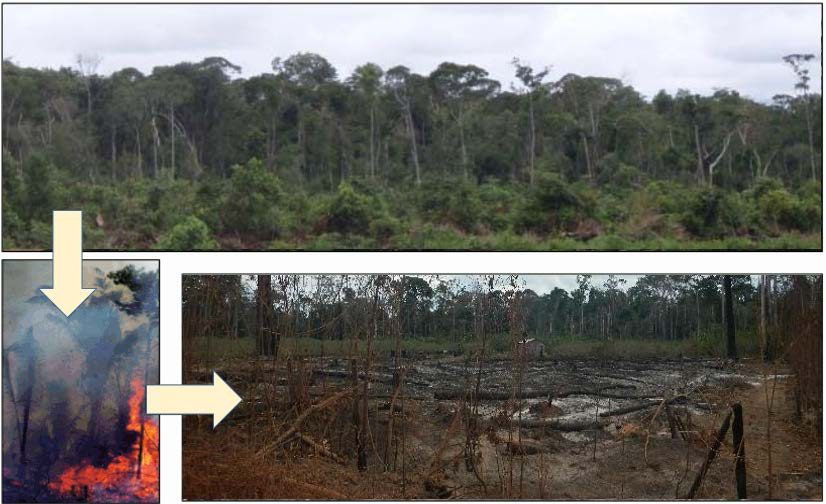
\includegraphics[width=0.99\linewidth]
                {./images/corte_e_queima.png}
                \caption{Deforestation by slash and cut (\textit{Corte e queima}).
                Source:~\cite{dealmeida2022}.}
            \end{figure}
        \end{column}
    \end{columns}
\end{frame}

\begin{frame}
    \frametitle{Amazon fire calendar}
    \begin{columns}
        \begin{column}{0.5\linewidth}
            \begin{itemize}
                \item Stratification of the Amazon basin according to the dry
                    season start and \/end.
                \item It uses the mean monthly rainfall (CHIRPS) from 1989 to
                    2019 over a 10 km grid.
                \item The dry season is made of the consecutive months with 
                    rainfall below 100 mm.
                \item Regions are neighborhoods of pixels with the same start
                    and end.
                \item Their results are available online
                    \href{https://zenodo.org/records/5706455}{online}.
            \end{itemize}
        \end{column}
        \begin{column}{0.5\linewidth}
            \begin{figure}[h]
                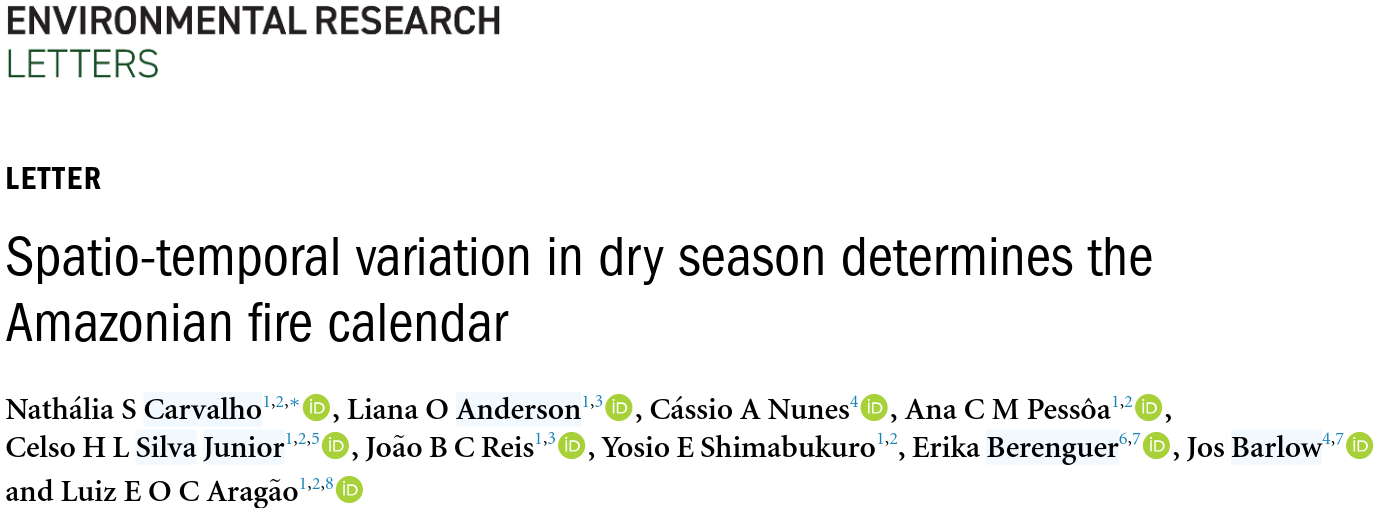
\includegraphics[width=0.79\linewidth]
                {./images/carvalho2021.png}
                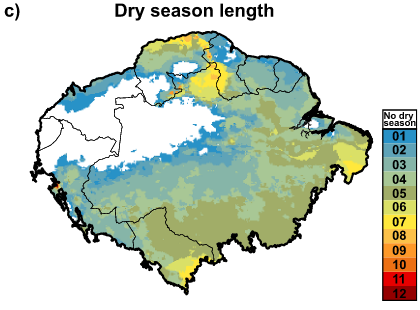
\includegraphics[width=0.69\linewidth]
                {./images/carvalho_fire_season_length.png}
                \caption{Source:~\cite{carvalho2021}.}
            \end{figure}
        \end{column}
    \end{columns}
\end{frame}

\section{Materials \& methods}

\begin{frame}
    \frametitle{Software}
    \begin{columns}
        \begin{column}{0.5\linewidth}
            \begin{itemize}
                \item R language~\cite{ihaka1996}.
                \item R packages \textit{dplyr} and \textit{ggplot2}.
                \item R packages for vector (\textit{sf}~\cite{pebesma2018})
                    and raster (\textit{terra}~\cite{hijmans2020}) data.
                \item R package \textit{sicegar} for double sigmoid
                    regression~\cite{caglar2018}.
                \item Analysis code available on
                    \href{https://github.com/albhasan/seasonmetrics}{GitHub}.
            \end{itemize}
        \end{column}
        \begin{column}{0.5\linewidth}
            \begin{figure}[h]
                
\includegraphics[width=0.35\linewidth]{./logos/Rlogo.png}
                
\includegraphics[width=0.29\linewidth]{./logos/sf_logo.png}
                
\includegraphics[width=0.25\linewidth]{./logos/terra_logo.png}\\
                
\includegraphics[width=0.24\linewidth]{./logos/dplyr.png}
                
\includegraphics[width=0.24\linewidth]{./logos/ggplot2_logo.png}
            \end{figure}
        \end{column}
    \end{columns}
\end{frame}

\begin{frame}
    \frametitle{Data}
    \begin{columns}
        \begin{column}{0.5\linewidth}
            \begin{itemize}
                \item We used fire data from VIIRS NPP.
            \end{itemize}
        \end{column}
        \begin{column}{0.5\linewidth}
            \begin{figure}
                %TODO: Add statistics: first and last fire, total number of fires.
                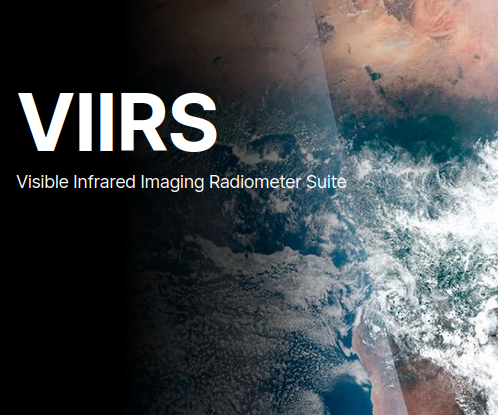
\includegraphics[width=0.9\linewidth]{./logos/viirs.png}
            \end{figure}
        \end{column}
    \end{columns}
\end{frame}

\subsection{Method 1: Peak and threshold}

\begin{frame}
    \frametitle{Peak and threshold}.
    \begin{columns}
        \begin{column}{0.5\linewidth}
            \begin{itemize}
                \item Proposed by Guilherme Mataveli.
                \item A season is a subset of contiguous months that host the
                    peak and at least 60\% of the total intensity
                    (observations) of a phenomenon.
            \end{itemize}
        \end{column}
        \begin{column}{0.5\linewidth}
            \begin{figure}[h]
                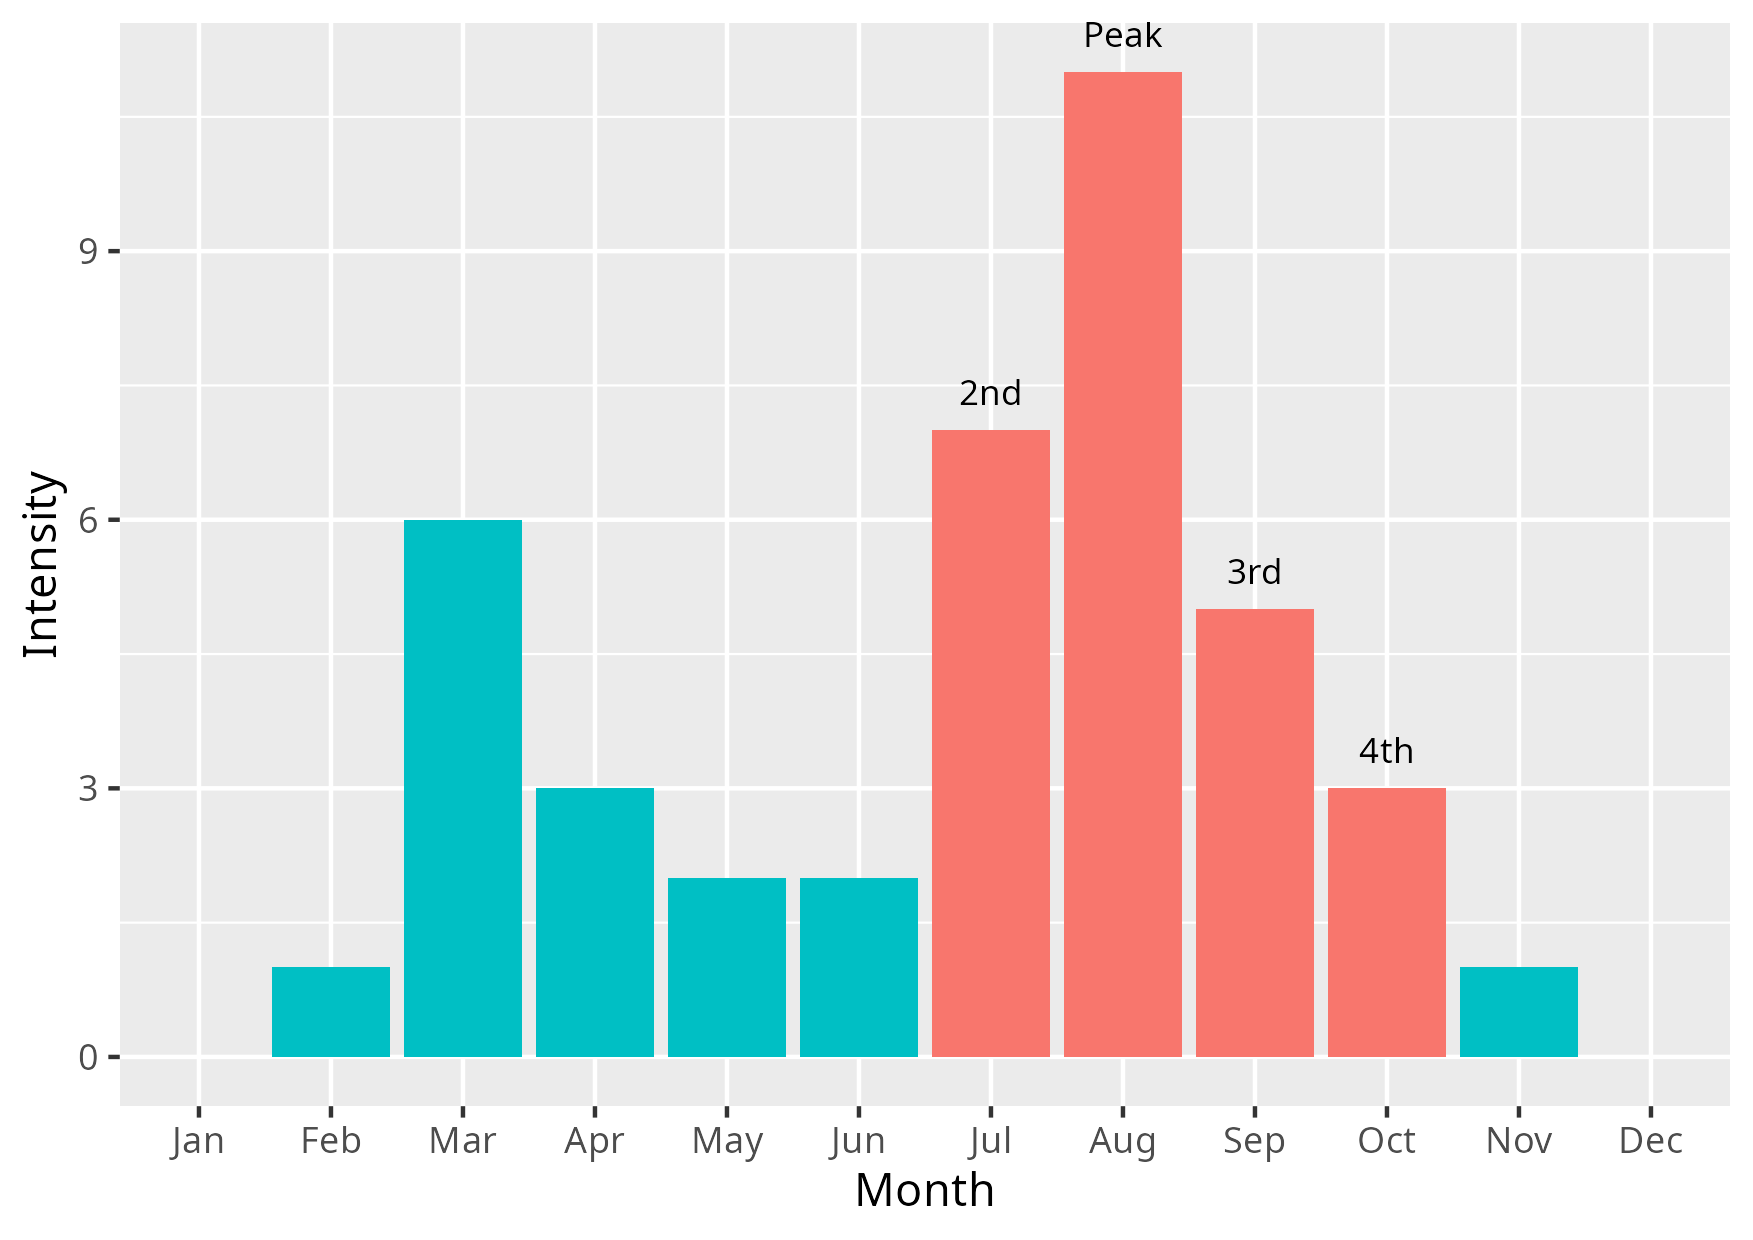
\includegraphics[width=0.99\linewidth]
                {./images/peak_thres_hist.png}
            \end{figure}
        \end{column}
    \end{columns}
\end{frame}

%\begin{frame}
%    \frametitle{Peak and threshold example}
%    \begin{tabular}{|c|r|}\hline
%        \bfseries Month & \bfseries GC
%        \csvreader[head to column names]
%        {./tables/monthly_counts.csv}{}
%        { \\\Month & \GC }
%        \\\hline
%    \end{tabular}
%\end{frame}

\begin{frame}
    \frametitle{Peak and threshold example}
    \begin{columns}
        \begin{column}{0.2\linewidth}
            \begin{tabular}{cr}
                \toprule
                \bfseries Month & \bfseries GC
                \csvreader[head to column names]
                {./tables/monthly_counts.csv}{}
                { \\\Month & \GC }
                \\\bottomrule
            \end{tabular}
        \end{column}
        \begin{column}{0.8\linewidth}
            \begin{figure}[h]
                \centering
                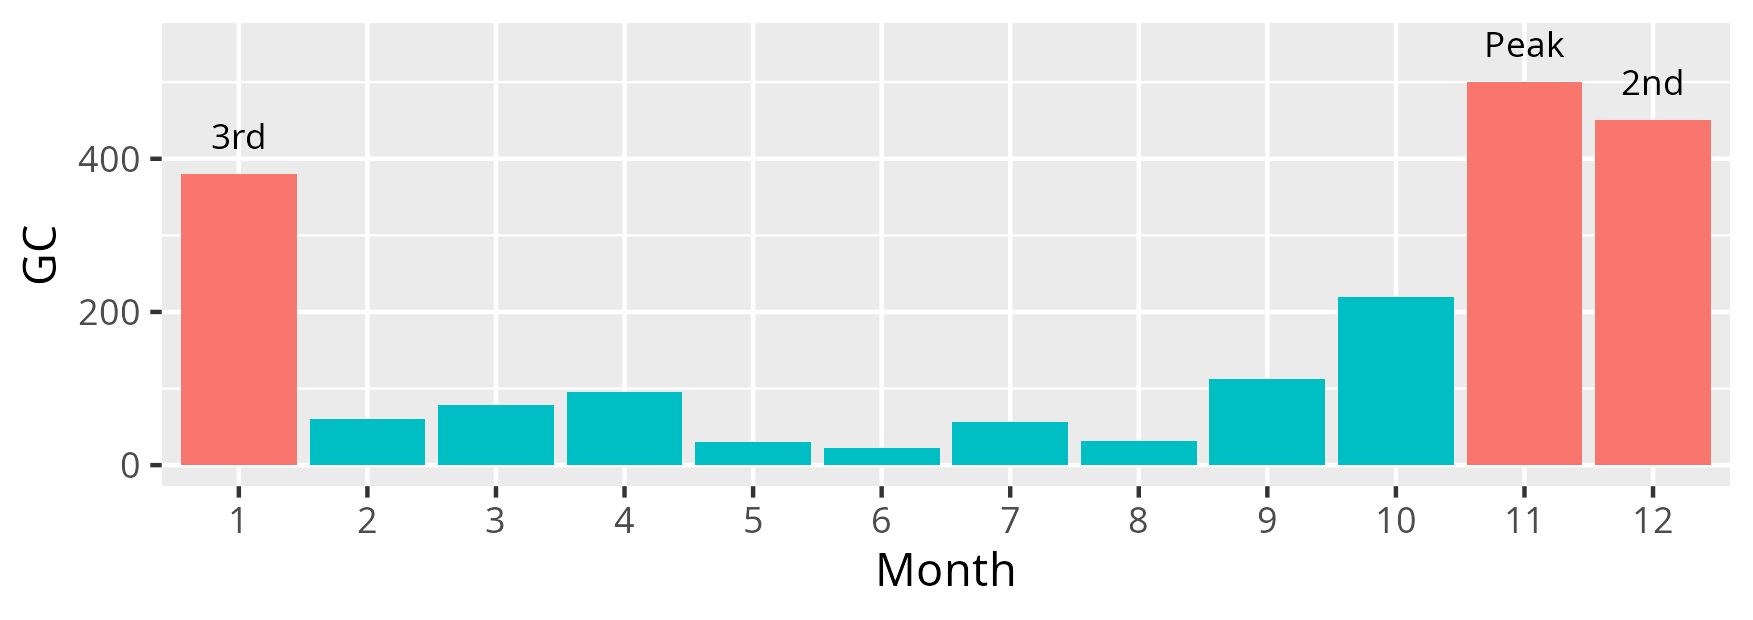
\includegraphics[width=0.89\linewidth]
                {./images/peak_thres_example.png}
            \end{figure}
            \begin{table}
                \centering
            \begin{tabular}{ccccr}
                \toprule
                \bfseries Iteration & \bfseries Test Months & \bfseries Chosen & \bfseries Season & \bfseries Cum. Sum
                \csvreader[head to column names]
                {./tables/iteration.csv}{}
                { \\\Iteration & \TestMonths & \Chosen & \Season & \CumSum}
                \\\bottomrule
            \end{tabular}
            \end{table}
        \end{column}
    \end{columns}
\end{frame}

\subsection{Method 2: Double sigmoidal}

\begin{frame}
    \frametitle{Double sigmoidal fitting}
    \begin{columns}
        \begin{column}{0.5\linewidth}
            \begin{itemize}
                \item Input data represents intensity measured over time.
                \item Growth happens in two phases: exponential intensity
                    increase until level off at a maximum level (first
                    sigmoid function); decay to a lower intensity or even zero
                    (second sigmoid).
                \item The midpoints are assumed as the start and end of the
                    season.
            \end{itemize}
        \end{column}
        \begin{column}{0.5\linewidth}
            \begin{figure}[h]
                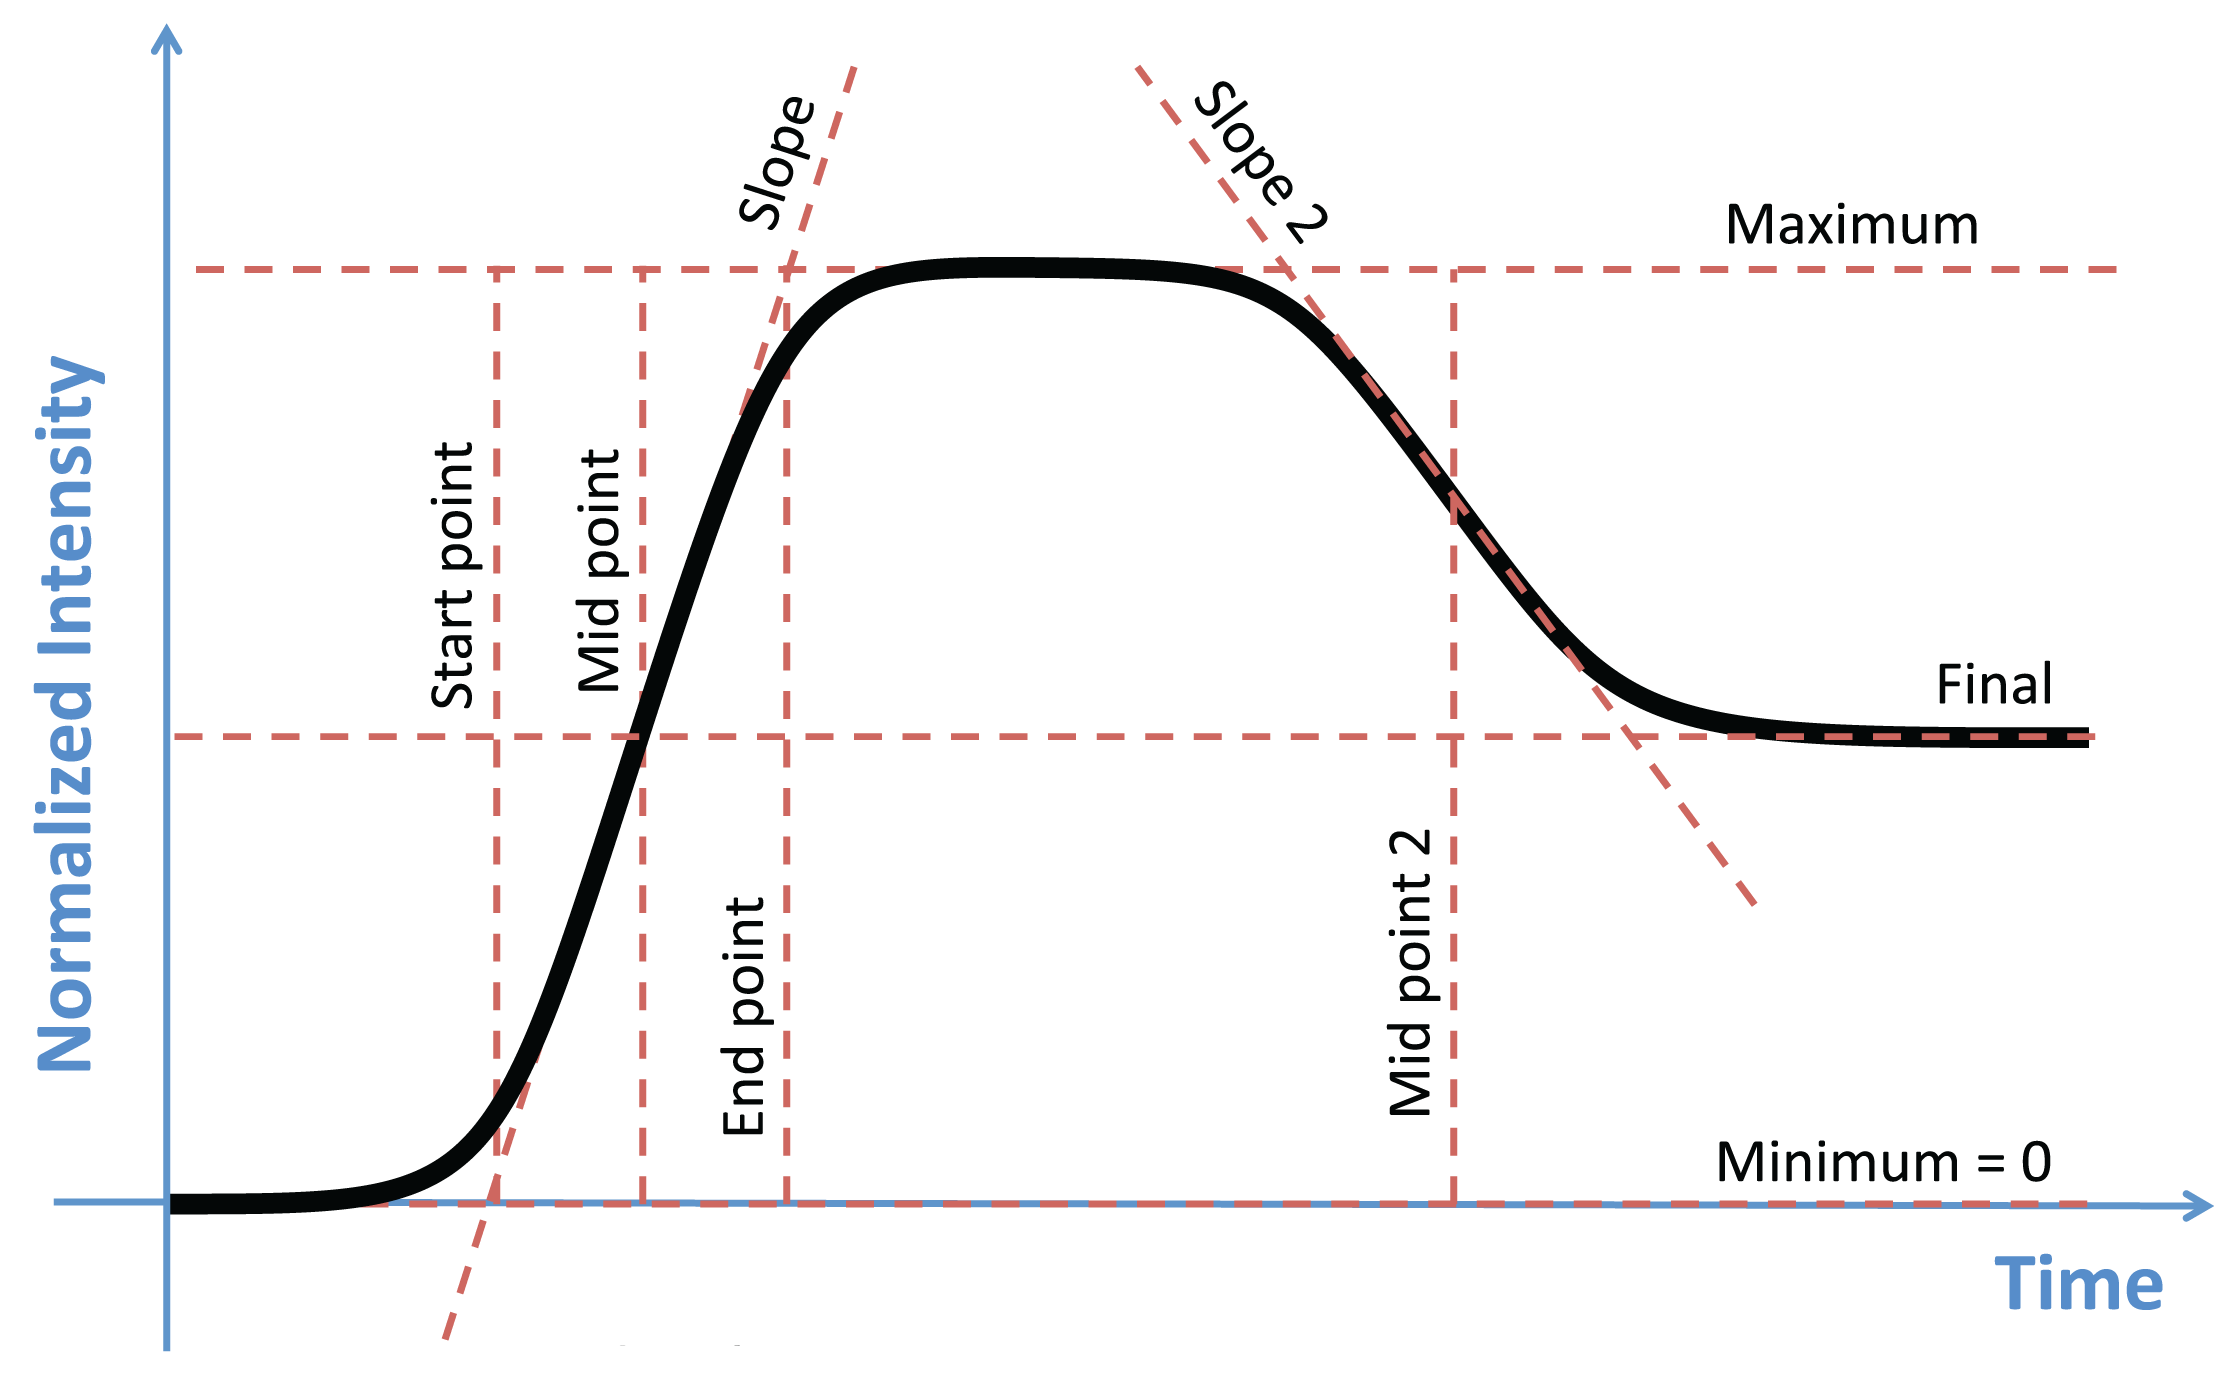
\includegraphics[width=0.99\linewidth]
                {./images/dsig_function.png}
                \caption{Source:~\cite{caglar2018}.}
            \end{figure}
        \end{column}
    \end{columns}
\end{frame}

\section{Results}

\begin{frame}
    \frametitle{Results}
    \begin{figure}[h]
        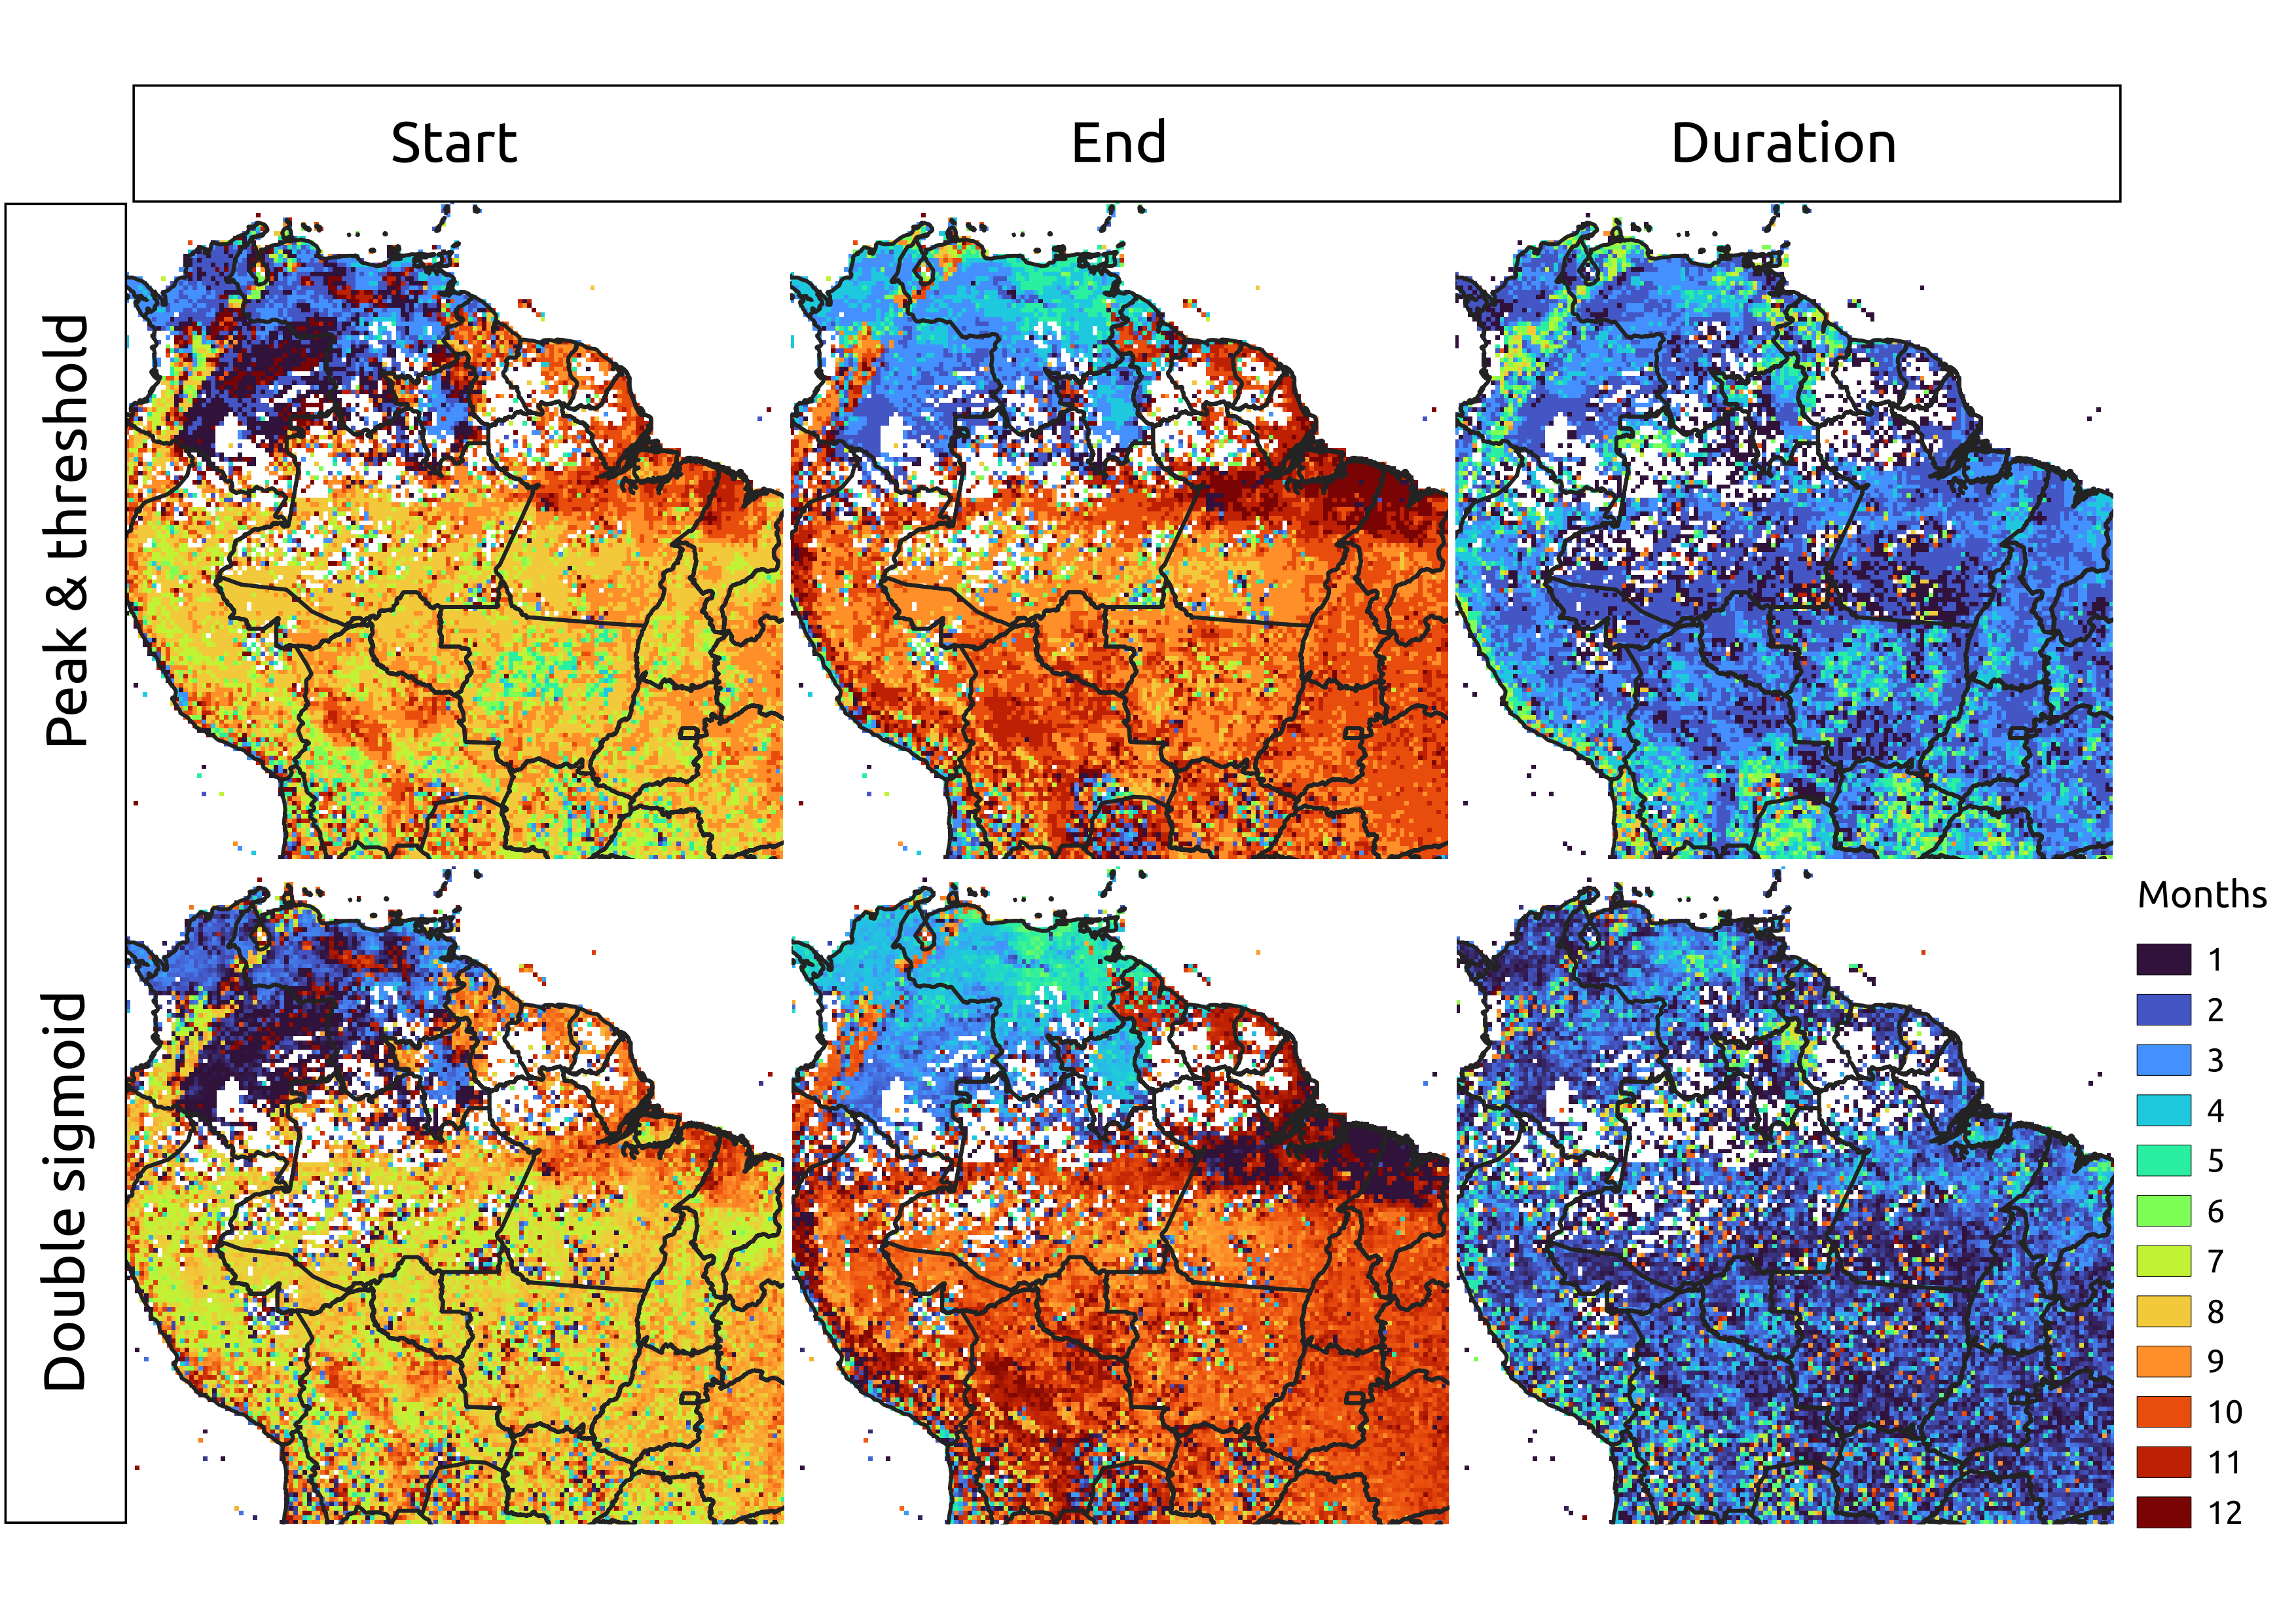
\includegraphics[width=0.75\linewidth]
        {./images/pthres_vs_dsig.png}
    \end{figure}
\end{frame}

\begin{frame}
    \frametitle{Result comparison}
    \begin{itemize}
        \item Carvalho et al., ~\cite{carvalho2021} is actually about the
            establishing the dry and rainy seasons rather than the fire season.
        \item They use the fire spots to validate their results.
        \item Instead, we're using the fire spots to estimate the fire season
            and use ~\cite{carvalho2021}, to validate them.
    \end{itemize}
\end{frame}

\begin{frame}
    \frametitle{Result comparison}
    \begin{figure}[h]
        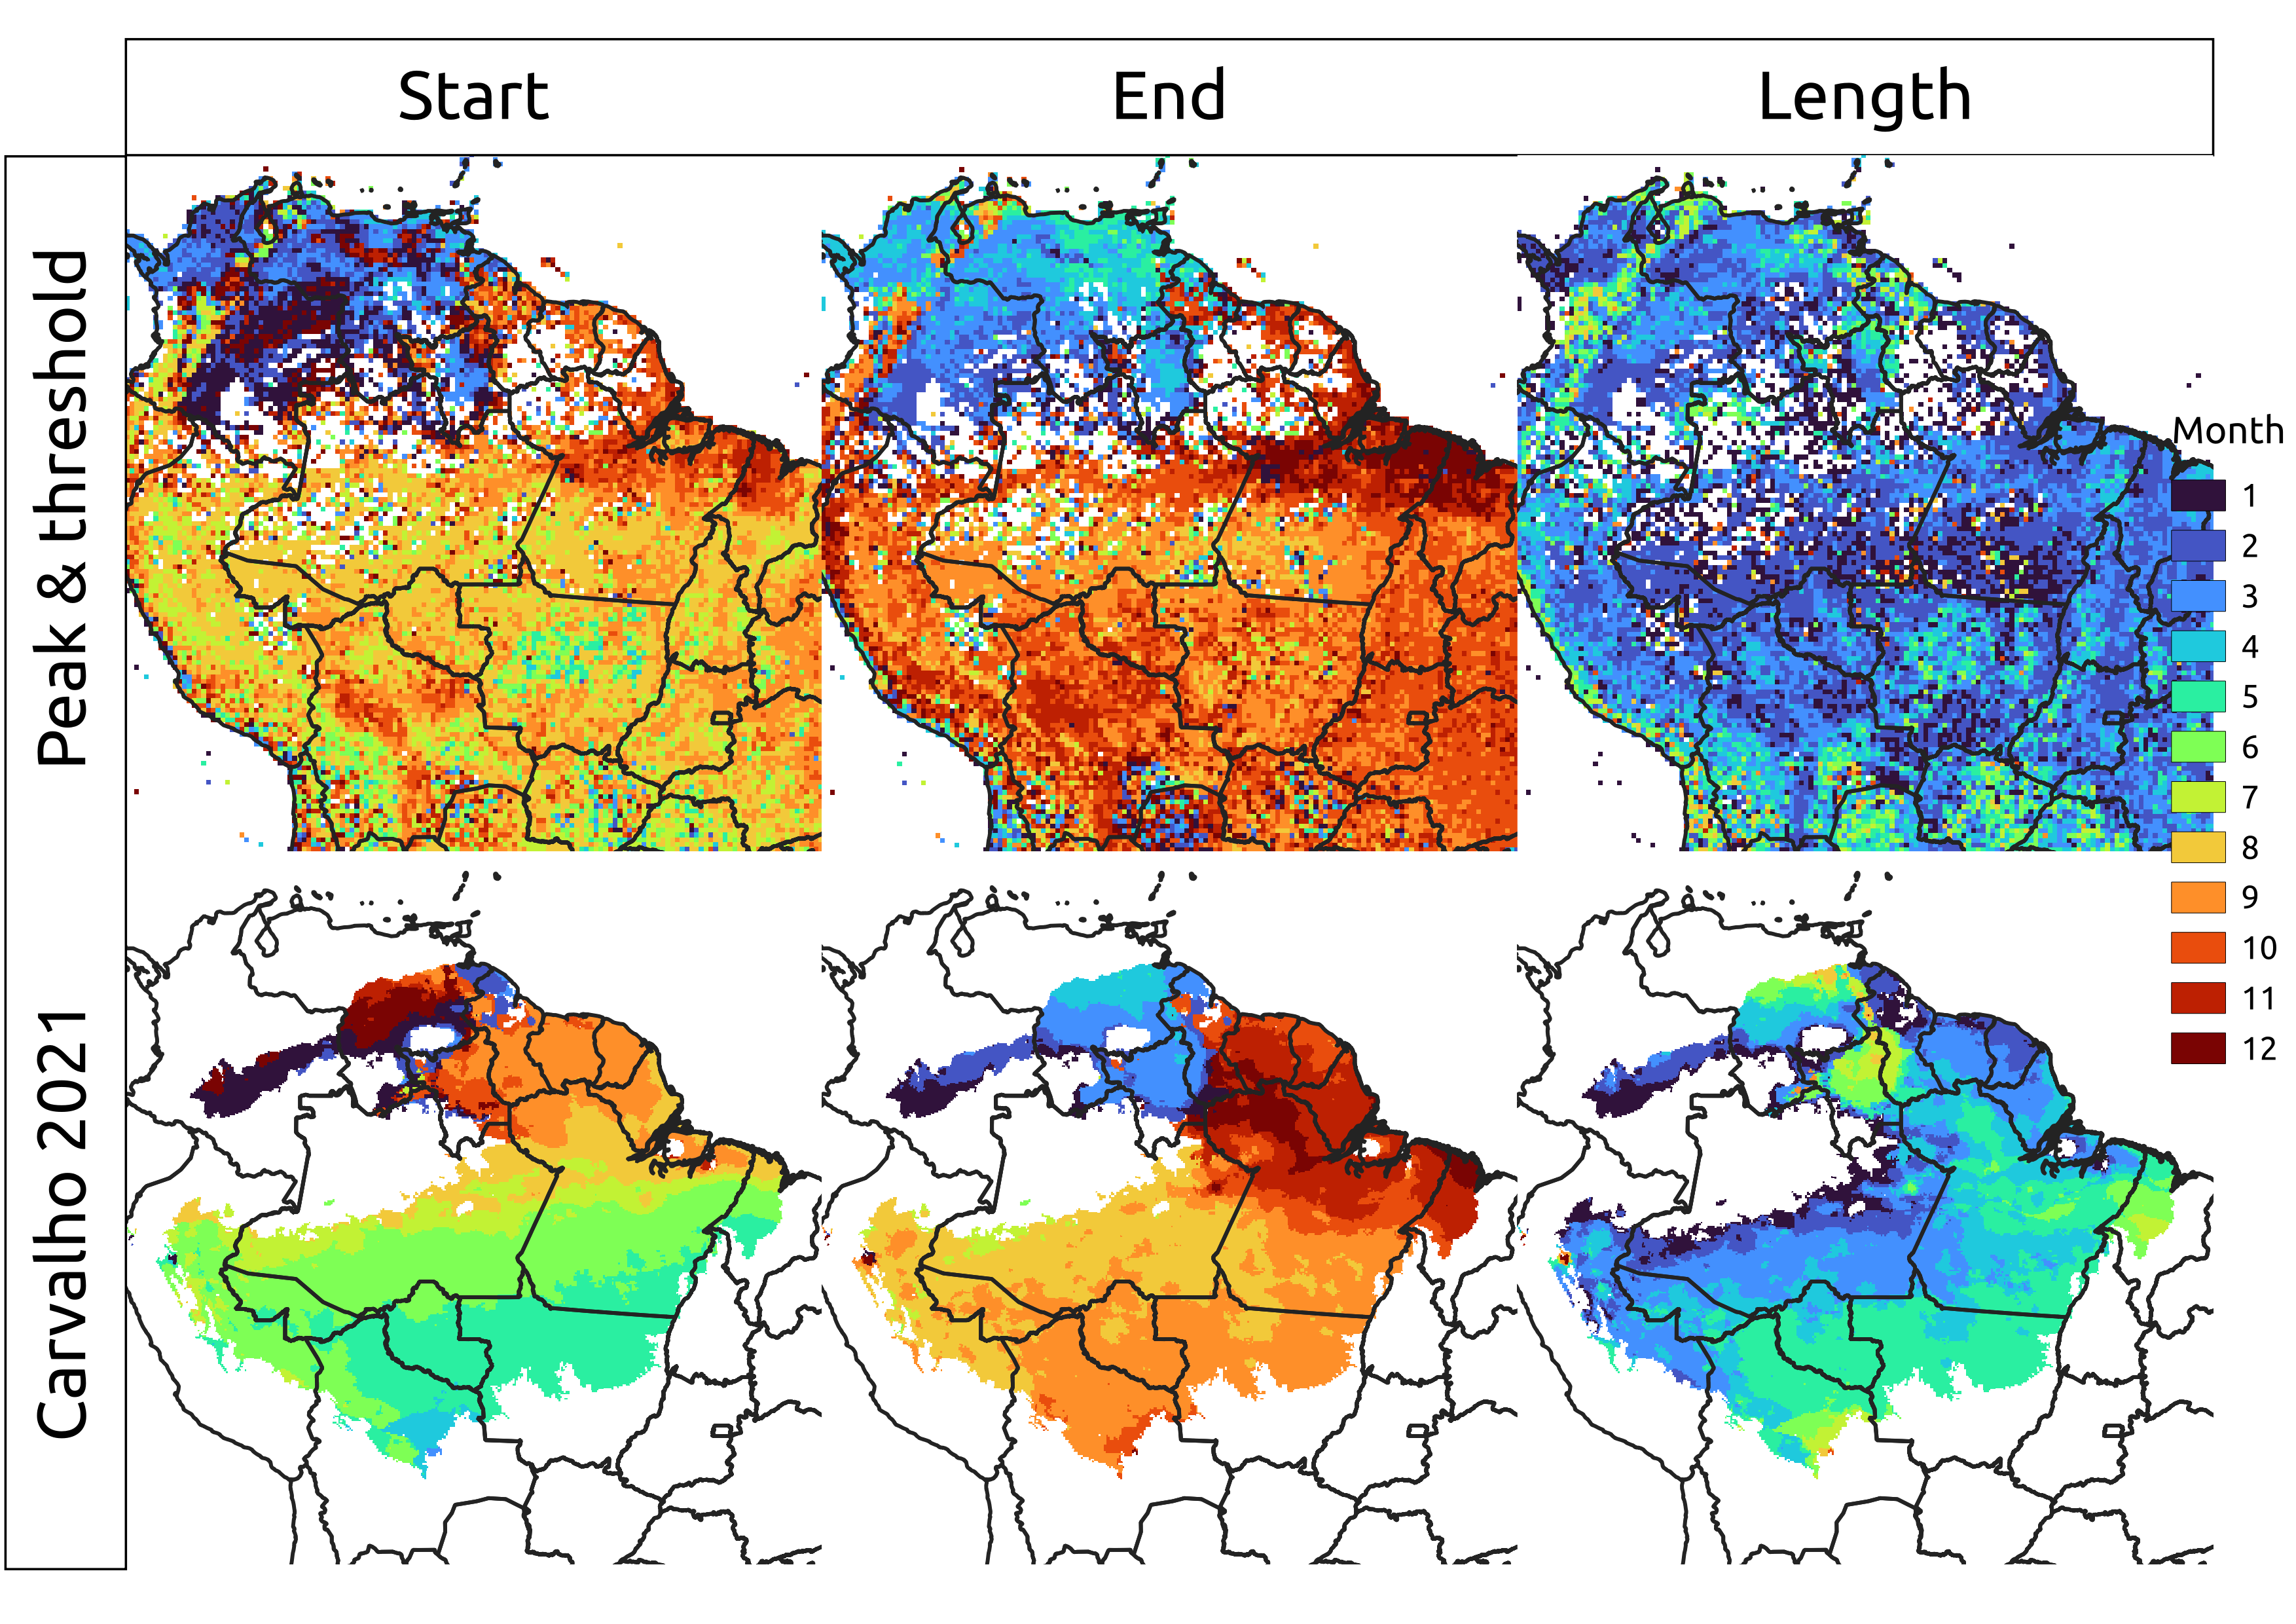
\includegraphics[width=0.75\linewidth]
        {./images/pthres_vs_carvalho2021.png}
    \end{figure}
\end{frame}

\section{Final remarks}

\begin{frame}
    \frametitle{Final remarks}
    \begin{columns}
        \begin{column}{0.5\linewidth}
            \begin{itemize}
                \item We ran both methods for the world.
                \item Both peak \& threshold and double sigmoid methods can be
                    employed to estimate season of Earth Observation phenomena 
                    besides fire.
                \item Source code available at
                    \url{https://github.com/albhasan/seasonmetrics}.
            \end{itemize}
        \end{column}
        \begin{column}{0.5\linewidth}
            \begin{figure}[h]
                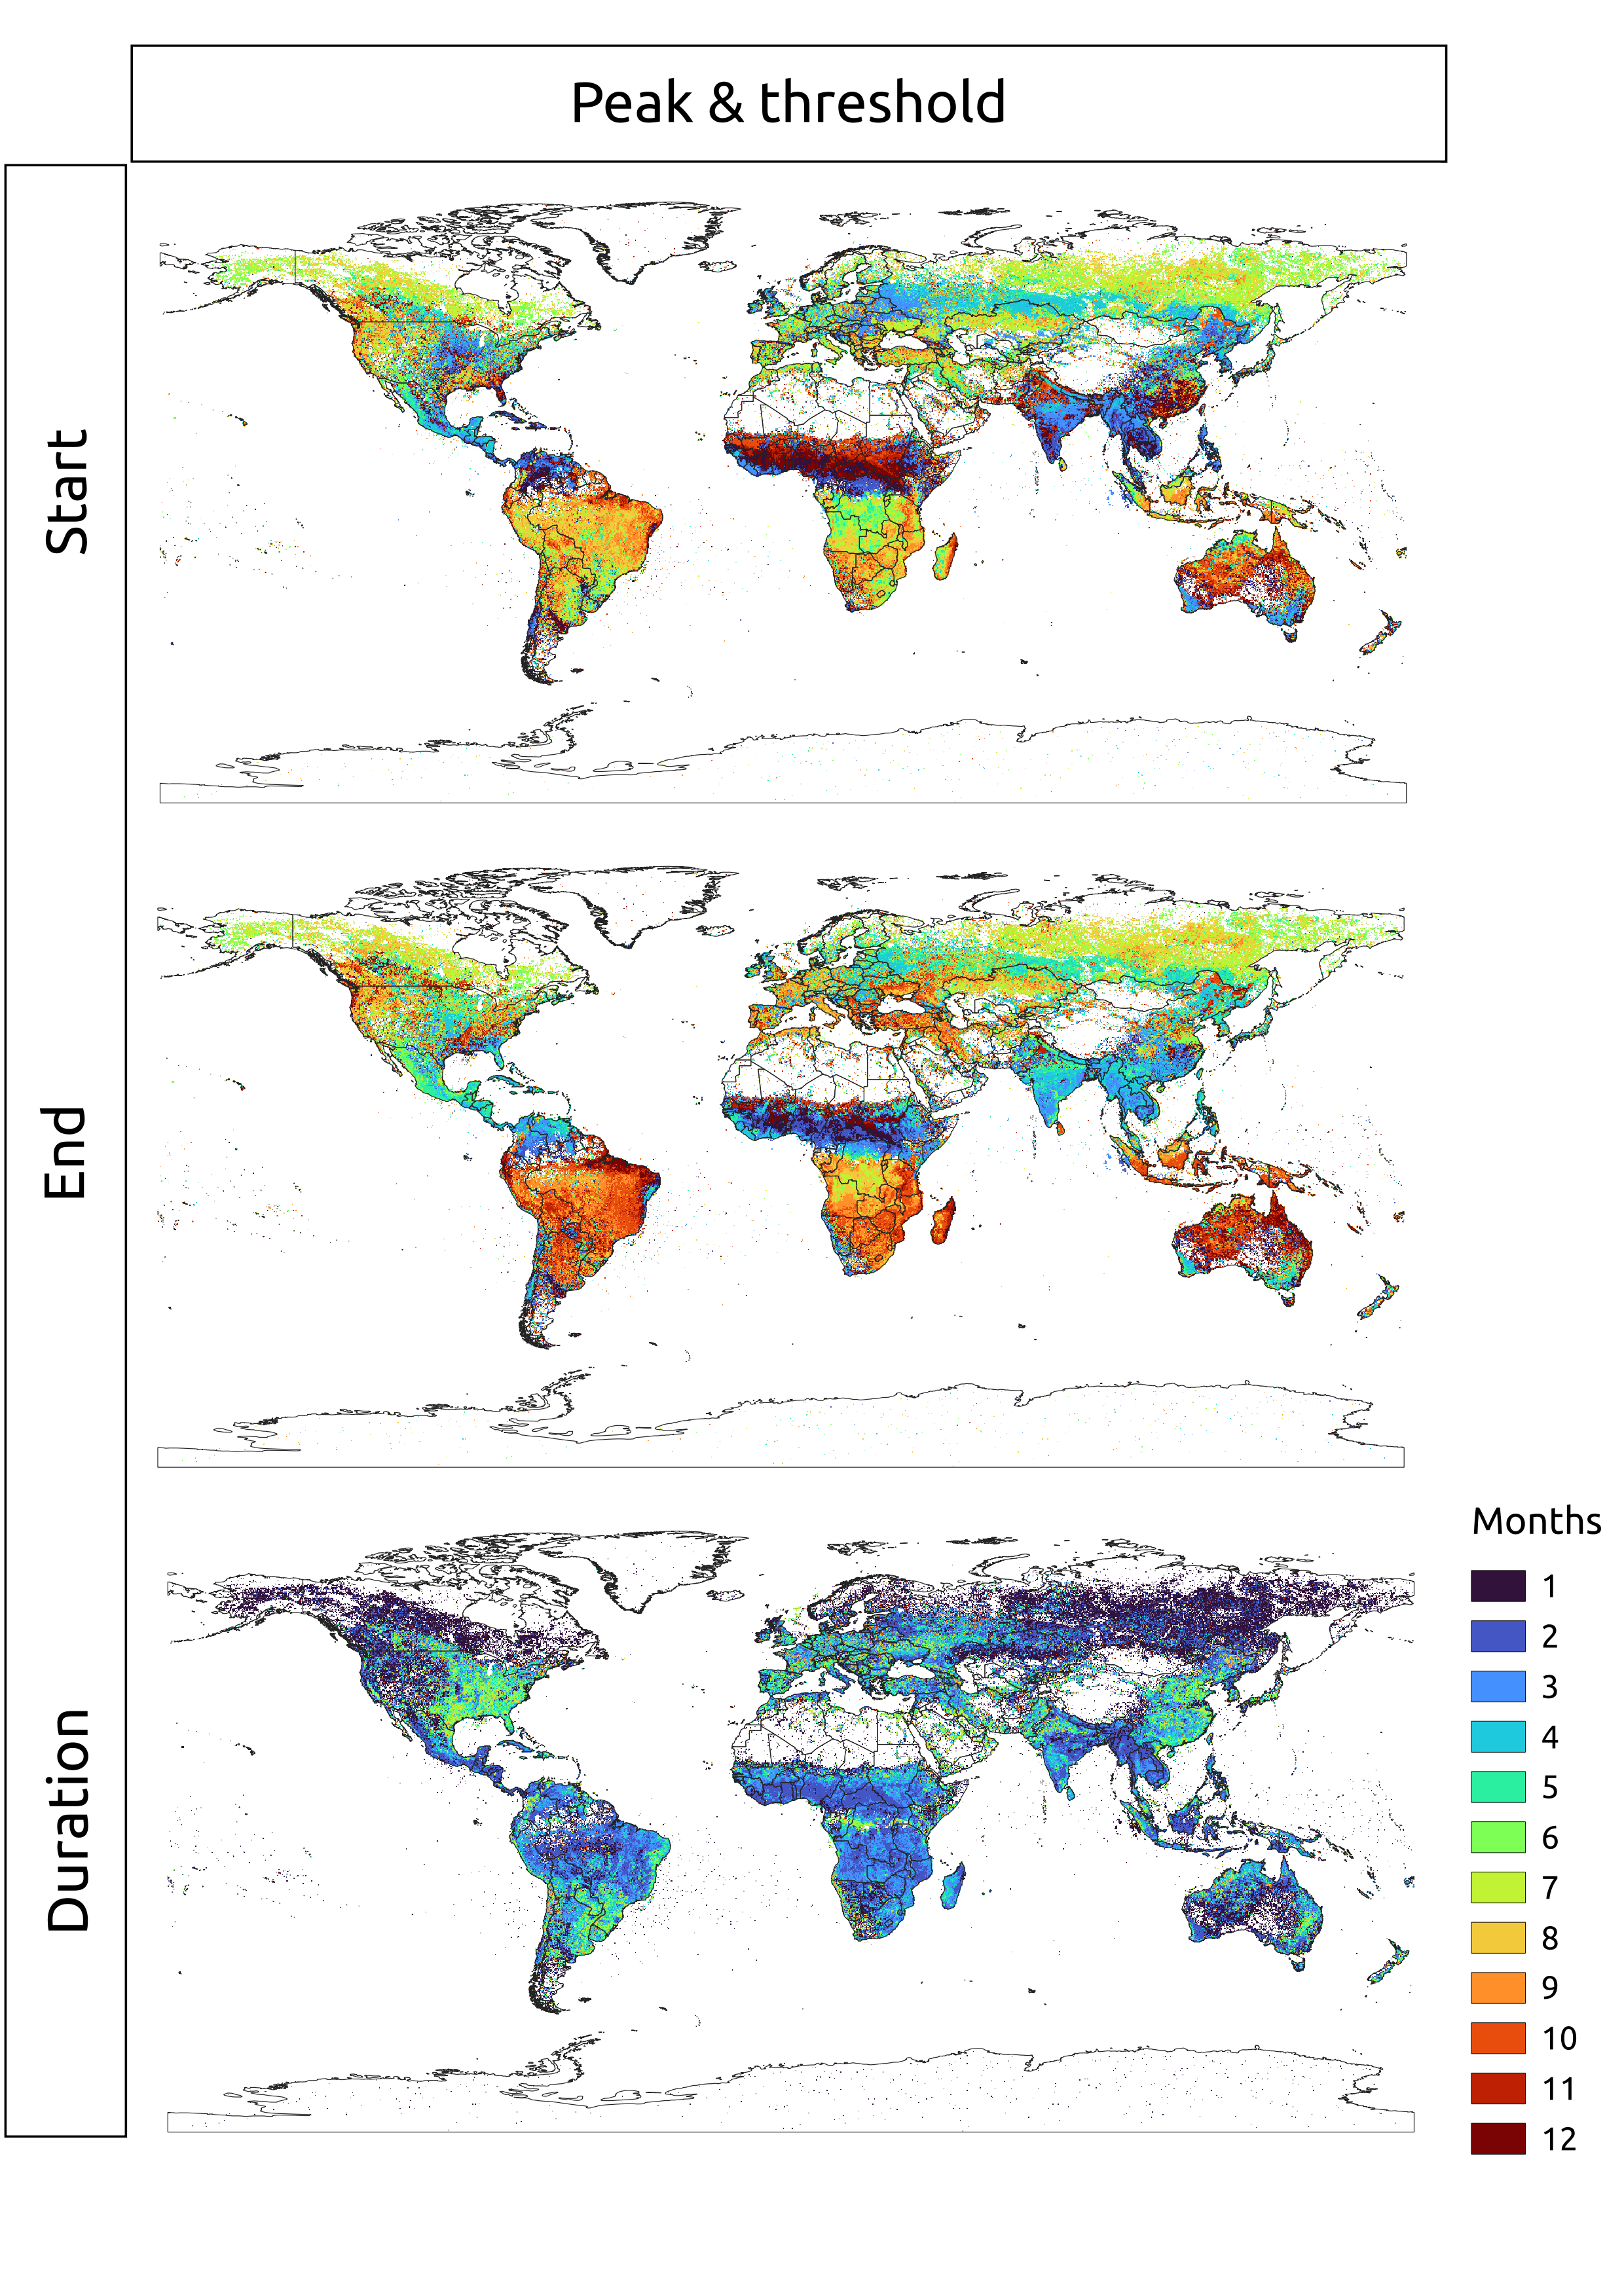
\includegraphics[width=0.99\linewidth]
                {./images/pthres_world.png}
                \caption{Length of the fire season using Peak \& Threshold.}
            \end{figure}
        \end{column}
    \end{columns}
\end{frame}

\begin{frame}[allowframebreaks]
    \frametitle{References}
    \bibliographystyle{amsalpha}
    \bibliography{seasonmetrics.bib}
\end{frame}

\end{document}
